\chapter{Geometría}

\index{geometría}

En los problemas geométricos, suele ser complicado afrontar el problema
tal que la solución se pueda implementar convenientemente y no existan
demasiados casos espciales.

Por ejemplo, considera el problema donde recibimos los vértices de un
cuadrilátero (un polígono con cuatro vértices), y nuestra tarea es calcular
su área. Por ejemplo, una entrada posible para el problema es la siguiente:

\begin{center}
    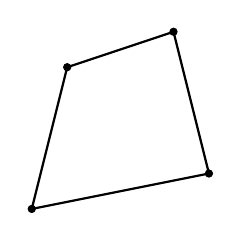
\begin{tikzpicture}[scale=0.45]

        \draw[fill] (6,2) circle [radius=0.1];
        \draw[fill] (5,6) circle [radius=0.1];
        \draw[fill] (2,5) circle [radius=0.1];
        \draw[fill] (1,1) circle [radius=0.1];
        \draw[thick] (6,2) -- (5,6) -- (2,5) -- (1,1) -- (6,2);
    \end{tikzpicture}
\end{center}
Una manera de resolver el problema es dividir el cuadrilátero en dos
triángulos a través de una línea recta entre dos vértices opuestos:
\begin{center}
    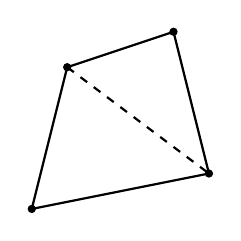
\begin{tikzpicture}[scale=0.45]

        \draw[fill] (6,2) circle [radius=0.1];
        \draw[fill] (5,6) circle [radius=0.1];
        \draw[fill] (2,5) circle [radius=0.1];
        \draw[fill] (1,1) circle [radius=0.1];

        \draw[thick] (6,2) -- (5,6) -- (2,5) -- (1,1) -- (6,2);
        \draw[dashed,thick] (2,5) -- (6,2);
    \end{tikzpicture}
\end{center}
Luego, podemos sumar las áreas de los triángulos. El área de un triángulo
puede calcularse, por ejemplo, utilizando la \key{fórmula de Herón}
%\footnote{Heron of Alexandria (c. 10--70) was a Greek mathematician.}
\[ \sqrt{s (s-a) (s-b) (s-c)},\]
donde $a$, $b$ y $c$ son las longitudes de los lados del triángulo y
$s=(a+b+c)/2$.
\index{fórmula de!Herón}

Esta es una manera posible de resolver el problema, pero hay un obstáculo:
¿\emph{cómo} dividimos el cuadrilátero en triángulos? Resulta que a veces no
podemos simplemente elegir dos vértices opuestos. Por ejemplo, en la siguiente
situación, la linea de división se encuentra \emph{fuera} del cuadrilátero:
\begin{center}
    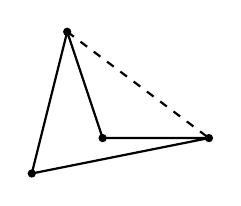
\begin{tikzpicture}[scale=0.45]

        \draw[fill] (6,2) circle [radius=0.1];
        \draw[fill] (3,2) circle [radius=0.1];
        \draw[fill] (2,5) circle [radius=0.1];
        \draw[fill] (1,1) circle [radius=0.1];
        \draw[thick] (6,2) -- (3,2) -- (2,5) -- (1,1) -- (6,2);

        \draw[dashed,thick] (2,5) -- (6,2);
    \end{tikzpicture}
\end{center}
Sin embargo, otra forma de trazar la linea sí nos sirve:
\begin{center}
    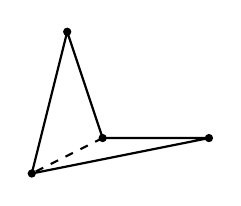
\begin{tikzpicture}[scale=0.45]

        \draw[fill] (6,2) circle [radius=0.1];
        \draw[fill] (3,2) circle [radius=0.1];
        \draw[fill] (2,5) circle [radius=0.1];
        \draw[fill] (1,1) circle [radius=0.1];
        \draw[thick] (6,2) -- (3,2) -- (2,5) -- (1,1) -- (6,2);

        \draw[dashed,thick] (3,2) -- (1,1);
    \end{tikzpicture}
\end{center}
Para un humano, está claro cuál de las dos líneas es la correcta, pero la
situación es difícil para una computadora.

De todos modos, resulta que hay otro método para resolver el problema
que es más conveniente para un programador: existe una fórmula general
\[x_1y_2-x_2y_1+x_2y_3-x_3y_2+x_3y_4-x_4y_3+x_4y_1-x_1y_4,\]
que calcula el área de un cuadrilátero cuyos vértices son
$(x_1,y_1)$,
$(x_2,y_2)$,
$(x_3,y_3)$ y
$(x_4,y_4)$.
Esta fórmula es fácil de implementar, no existen casos especiales, e incluso
podemos generalizarla a \emph{todos} los polígonos (Capítulo 29.3).

\section{Números complejos}

\index{número complejo}
\index{punto}
\index{vector}

Un \key{número complejo} es un número en la forma $x+y i$, donde
$i = \sqrt{-1}$ es la \key{unidad imaginaria}. Una interpretación geométrica
de un número complejo es que representa un punto bidimensional $(x,y)$ o un
vector desde el origen hasta el punto $(x,y)$.

Por ejemplo, $4+2i$ corresponde al siguiente punto y vector:

\begin{center}
    \begin{tikzpicture}[scale=0.45]

        \draw[->,thick] (-5,0)--(5,0);
        \draw[->,thick] (0,-5)--(0,5);

        \draw[fill] (4,2) circle [radius=0.1];
        \draw[->,thick] (0,0)--(4-0.1,2-0.1);

        \node at (4,2.8) {$(4,2)$};
    \end{tikzpicture}
\end{center}

\index{complex@\texttt{complex}}

La clase para números complejos de C++, \texttt{complex}, es útil al resolver
problemas geométricos. Utilizando esta clase, podemos representar puntos y
vectores como números complejos y hacer uso de herramientas útiles en
la geometría computacional.

En el siguiente código, \texttt{C} es el tipo de una coordenada y \texttt{P}
representa un punto o vector. Adicionalmente, el código define las macros
\texttt{X} e \texttt{Y} que podemos utilizar para acceder a las coordenadas
$x$ e $y$ representadas por un número complejo.

\begin{lstlisting}
typedef long long C;
typedef complex<C> P;
#define X real()
#define Y imag()
\end{lstlisting}

Por ejemplo, el siguiente código define un punto $p=(4,2)$ y muestra sus
coordenadas x e y:

\begin{lstlisting}
P punto = { 4, 2 };
cout << punto.X << " " << punto.Y; // 4 2
\end{lstlisting}

El siguiente código define los vectores $v=(3,1)$ y $u=(2,2)$, y luego calcula
la suma $s=v+u$.

\begin{lstlisting}
P v = { 3, 1 };
P u = { 2, 2 };
P s = v + u;
cout << s.X << " " << s.Y; // 5 3
\end{lstlisting}

En la práctica, un tipo de coordenada apropiado es usualmente el
\texttt{long long} (número entero) o \texttt{long double} (número real).
Es una buena idea utilizar enteros siempre y cuando sea posible, porque
esto garantiza la exactitud de nuestros cálculos. Si debemos utilizar números
reales, también debemos tener en cuenta errores de precisión al comparar
valores. Una forma segura de revisar si los números reales $a$ y $b$ son
iguales es compararlos utilizando $|a-b|<\varepsilon$, donde $\varepsilon$
es un número pequeño (por ejemplo, $\varepsilon=10^{-9}$).

\subsubsection*{Funciones}

En los siguientes ejemplos, el tipo de coordenada es \texttt{long double}.

La función $\texttt{abs}(v)$ calcula la longitud de un vector $v$ con la
fórmula $\sqrt{x^2+y^2}$. Esta función también puede utilizarse para calcular
la distancia entre los puntos $(x_1,y_1)$ y $(x_2,y_2)$, porque esta es igual
a la longitud del vector $(x_2-x_1,y_2-y_1)$.

El siguiente código calcula la distancia entre los puntos $(4,2)$ y $(3,-1)$:
\begin{lstlisting}
P a = { 4, 2 };
P b = { 3, -1 };
cout << abs(b - a); // 3.16228
\end{lstlisting}

La función $\texttt{arg}(v)$ calcula el ángulo de un vector $v$ con
respecto al eje x. Esta función devuelve el ángulo en radianes, donde $r$
radianes equivale a $180 r/\pi$ grados. El ángulo de un vector que apunta
a la derecha es 0, y el ángulo aumenta en sentido antihorario y disminuye
en sentido horario.

La función $\texttt{polar}(s,a)$ construye un vector cuya longitud es $s$
y que apunta a un ángulo $a$. Un vector puede rotarse por un ángulo $a$ si
lo multiplicamos por un vector con longitud 1 y ángulo $a$.

El siguiente código calcula el ángulo del vector $(4,2)$, lo rota medio
radián en sentido antihorario, y luego vuelve a calcular el ángulo:

\begin{lstlisting}
P v = { 4, 2 };
cout << arg(v); // 0.463648
v *= polar(1.0, 0.5);
cout << arg(v); // 0.963648
\end{lstlisting}

\section{Puntos y líneas}

\index{producto vectorial}

El \key{producto vectorial} (o \textit{producto cruz}) $a \times b$ de dos
vectores $a=(x_1,y_1)$ y $b=(x_2,y_2)$ se calcula usando la fórmula
$x_1 y_2 - x_2 y_1$. El producto vectorial nos dice si $b$ gira hacia la
izquierda (resultado positivo), no gira (cero), o gira hacia la derecha
(resultado negativo), cuando es colocado directamente tras $a$.

La siguiente imagen ilustra estos tres casos:
\begin{center}
    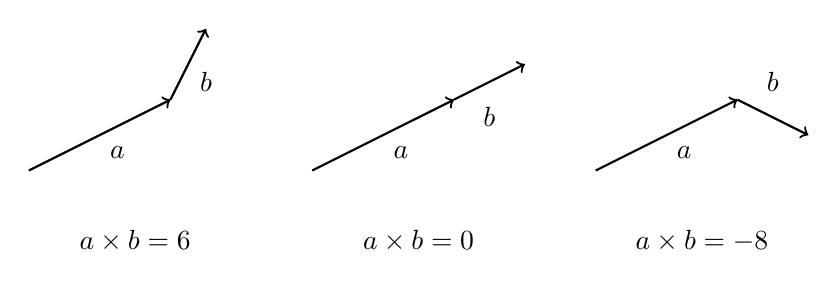
\begin{tikzpicture}[scale=0.45]

        \draw[->,thick] (0,0)--(4,2);
        \draw[->,thick] (4,2)--(4+1,2+2);

        \node at (2.5,0.5) {$a$};
        \node at (5,2.5) {$b$};

        \node at (3,-2) {$a \times b = 6$};

        \draw[->,thick] (8+0,0)--(8+4,2);
        \draw[->,thick] (8+4,2)--(8+4+2,2+1);

        \node at (8+2.5,0.5) {$a$};
        \node at (8+5,1.5) {$b$};

        \node at (8+3,-2) {$a \times b = 0$};

        \draw[->,thick] (16+0,0)--(16+4,2);
        \draw[->,thick] (16+4,2)--(16+4+2,2-1);

        \node at (16+2.5,0.5) {$a$};
        \node at (16+5,2.5) {$b$};

        \node at (16+3,-2) {$a \times b = -8$};
    \end{tikzpicture}
\end{center}

\noindent
Por ejemplo, en el primer caso $a=(4,2)$ y $b=(1,2)$. El siguiente código
calcula el producto vectorial usando la clase \texttt{complex}:

\begin{lstlisting}
P a = { 4, 2 };
P b = { 1, 2 };
C p = (conj(a) * b).Y; // 6
\end{lstlisting}

Este código funciona porque la función \texttt{conj} nega la coordenada $y$
de un vector, y cuando los vectores $(x_1,-y_1)$ y $(x_2,y_2)$ se multiplican,
la coordenada $y$ del resultado es $x_1 y_2 - x_2 y_1$.

\subsubsection{Ubicación de un punto}

Podemos usar el producto vectorial para revisar si un punto se ubica en
el lado izquierdo o derecho de una línea. Digamos que la línea cruza los puntos
$s_1$ y $s_2$, estamos mirando del punto $s_1$ a $s_2$ y el punto a ubicar
es $p$.

Por ejemplo, en la siguiente imagen, $p$ se encuentra en el lado izquierdo
de la línea:
\begin{center}
    \begin{tikzpicture}[scale=0.45]
        \draw[dashed,thick,->] (0,-3)--(12,6);
        \draw[fill] (4,0) circle [radius=0.1];
        \draw[fill] (8,3) circle [radius=0.1];
        \draw[fill] (5,3) circle [radius=0.1];
        \node at (4,-1) {$s_1$};
        \node at (8,2) {$s_2$};
        \node at (5,4) {$p$};
    \end{tikzpicture}
\end{center}

El producto vectorial $(p-s_1) \times (p-s_2)$ nos dice la ubicación del
punto $p$. Si el resultado es positivo, $p$ se encuentra en el lado izquierdo,
y si el resultado es negativo, $p$ se encuentra en el lado derecho. Finalmente,
si el resultado es cero, los puntos $s_1$, $s_2$, y $p$ se encuentran en la
misma línea.

\subsubsection{Intersección de segmentos}

\index{intersección de segmentos}

Ahora veremos el problema de revisar si dos segmentos $\overline{ab}$ y
$\overline{cd}$ se intersecan. Los casos posibles son:

\textit{Caso 1:}
Los segmentos están en la misma línea y se superponen. En este caso, hay un
número infinito de puntos de intersección. Por ejemplo, en la siguiente imagen,
todos los puntos entre $c$ y $b$ son de intersección:
\begin{center}
    \begin{tikzpicture}[scale=0.9]
        \draw (1.5,1.5)--(6,3);
        \draw (0,1)--(4.5,2.5);
        \draw[fill] (0,1) circle [radius=0.05];
        \node at (0,0.5) {$a$};
        \draw[fill] (1.5,1.5) circle [radius=0.05];
        \node at (6,2.5) {$d$};
        \draw[fill] (4.5,2.5) circle [radius=0.05];
        \node at (1.5,1) {$c$};
        \draw[fill] (6,3) circle [radius=0.05];
        \node at (4.5,2) {$b$};
    \end{tikzpicture}
\end{center}

En este caso, podemos usar el producto vectorial para revisar si todos
los puntos se encuentran en la misma línea. Luego de esto, podemos ordenar
los puntos y revisar si los segmentos se superponen entre sí.

\textit{Caso 2:}
Los segmentos tienen un vértice en común, que es el único punto de
intersección. Por ejemplo, en la siguiente imagen el punto de intersección
es $b=c$:

\begin{center}
    \begin{tikzpicture}[scale=0.9]
        \draw (0,0)--(4,2);
        \draw (4,2)--(6,1);
        \draw[fill] (0,0) circle [radius=0.05];
        \draw[fill] (4,2) circle [radius=0.05];
        \draw[fill] (6,1) circle [radius=0.05];

        \node at (0,0.5) {$a$};
        \node at (4,2.5) {$b=c$};
        \node at (6,1.5) {$d$};
    \end{tikzpicture}
\end{center}

Este caso es simple de revisar, porque solo existen cuatro posibilidades
para el punto de intersección: $a=c$, $a=d$, $b=c$, o $b=d$.

\textit{Caso 3:}
Hay exactamente un punto de intersección, que no es un vértice de ninguno de
los segmentos. En la siguiente imagen, el punto $p$ es el de intersección:
\begin{center}
    \begin{tikzpicture}[scale=0.9]
        \draw (0,1)--(6,3);
        \draw (2,4)--(4,0);
        \draw[fill] (0,1) circle [radius=0.05];
        \node at (0,0.5) {$c$};
        \draw[fill] (6,3) circle [radius=0.05];
        \node at (6,2.5) {$d$};
        \draw[fill] (2,4) circle [radius=0.05];
        \node at (1.5,3.5) {$a$};
        \draw[fill] (4,0) circle [radius=0.05];
        \node at (4,-0.4) {$b$};
        \draw[fill] (3,2) circle [radius=0.05];
        \node at (3,1.5) {$p$};
    \end{tikzpicture}
\end{center}

En este caso, los segmentos se intersecan exactamente cuando ambos puntos
$c$ y $d$ se encuentran en diferentes lados de una línea a través de $a$ y
$b$, y los puntos $a$ y $b$ están en diferentes lados de una línea a través
de $c$ y $d$. Podemos utilizar el producto vectorial para revisar esto.

\subsubsection{Distancia entre punto y línea}

Otra función del producto vectorial es que el área de un triángulo puede
calcularse utilizando la fórmula \[\frac{| (a-c) \times (b-c) |}{2},\]
donde $a$, $b$, y $c$ son los vértices del triángulo. Usando este hecho,
podemos derivar una fórmula para calcular la distancia más corta entre
un punto y una línea. Por ejemplo, en la siguiente imagen $d$ es la
distancia más corta entre el punto $p$ y la línea definida por los puntos
$s_1$ y $s_2$:
\begin{center}
    \begin{tikzpicture}[scale=0.75]
        \draw (-2,-1)--(6,3);
        \draw[dashed] (1,4)--(2.40,1.2);
        \node at (0,-0.5) {$s_1$};
        \node at (4,1.5) {$s_2$};
        \node at (0.5,4) {$p$};
        \node at (2,2.7) {$d$};
        \draw[fill] (0,0) circle [radius=0.05];
        \draw[fill] (4,2) circle [radius=0.05];
        \draw[fill] (1,4) circle [radius=0.05];
    \end{tikzpicture}
\end{center}

El área de un triángulo cuyos vértices son $s_1$, $s_2$, y $p$ puede
calcularse de dos maneras: es a la vez $\frac{1}{2} |s_2-s_1| d$ y
$\frac{1}{2} ((s_1-p) \times (s_2-p))$. Por ende, la distancia mínima es
\[ d = \frac{(s_1-p) \times (s_2-p)}{|s_2-s_1|} .\]

\subsubsection{Punto dentro de un polígono}

Ahora veremos el problema de revisar si un punto se encuentra ubicado dentro
o fuera de un polígono. Por ejemplo, en la siguiente imagen el punto $a$ está
dentro del polígono y el punto $b$ está fuera.

\begin{center}
    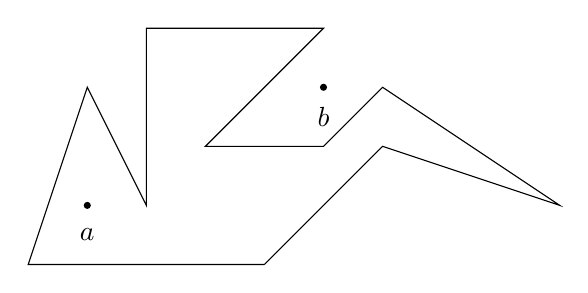
\begin{tikzpicture}[scale=0.75]
        %\draw (0,0)--(2,-2)--(3,1)--(5,1)--(2,3)--(1,2)--(-1,2)--(1,4)--(-2,4)--(-2,1)--(-3,3)--(-4,0)--(0,0);
        \draw (0,0)--(2,2)--(5,1)--(2,3)--(1,2)--(-1,2)--(1,4)--(-2,4)--(-2,1)--(-3,3)--(-4,0)--(0,0);

        \draw[fill] (-3,1) circle [radius=0.05];
        \node at (-3,0.5) {$a$};
        \draw[fill] (1,3) circle [radius=0.05];
        \node at (1,2.5) {$b$};
    \end{tikzpicture}
\end{center}

Una manera conveniente de resolver el problema es enviar un \emph{rayo} del
punto a alguna dirección arbitraria y calcular el número de veces que toca
los bordes del polígono. Si este número es impar, el punto se encuentra
adentro, y si el número es par, se encuentra afuera.

\begin{samepage}
    Por ejemplo, podemos enviar los siguientes rayos:
    \begin{center}
        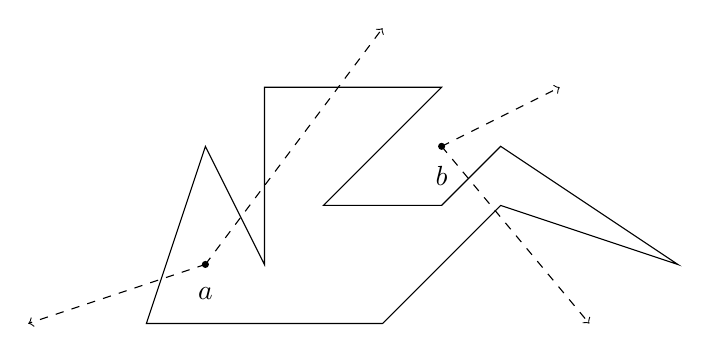
\begin{tikzpicture}[scale=0.75]
            \draw (0,0)--(2,2)--(5,1)--(2,3)--(1,2)--(-1,2)--(1,4)--(-2,4)--(-2,1)--(-3,3)--(-4,0)--(0,0);

            \draw[fill] (-3,1) circle [radius=0.05];
            \node at (-3,0.5) {$a$};
            \draw[fill] (1,3) circle [radius=0.05];
            \node at (1,2.5) {$b$};

            \draw[dashed,->] (-3,1)--(-6,0);
            \draw[dashed,->] (-3,1)--(0,5);

            \draw[dashed,->] (1,3)--(3.5,0);
            \draw[dashed,->] (1,3)--(3,4);
        \end{tikzpicture}
    \end{center}
\end{samepage}

Los rayos de $a$ tocan 1 y 3 veces al polígono, así que está adentro.
Correspondientemente, los rayos de $b$ tocan 0 y 2 veces al polígono, por
lo que $b$ está afuera.

\section{Área de un polígono}

\index{fórmula de!Gauss}

Una fórmula general para calcular el área de un polígono, a veces llamada la
\key{fórmula de Gauss}, es la siguiente:
\[\frac{1}{2} \left|\,\sum_{i=1}^{n-1} \left(p_i \times p_{i+1}\right)\,\right| =
    \frac{1}{2} \left|\,\sum_{i=1}^{n-1} \left(x_i y_{i+1} - x_{i+1} y_i\right)\,\right|. \]
Aquí los vértices son $p_1=(x_1,y_1), p_2=(x_2,y_2), \ldots, p_n=(x_n,y_n)$
en un orden tal que $p_i$ y $p_{i+1}$ son vértices adyacentes en el borde del
polígono, y el primer y último vértice es el mismo, o sea, $p_1=p_n$.

Por ejemplo, el área del polígono
\begin{center}
    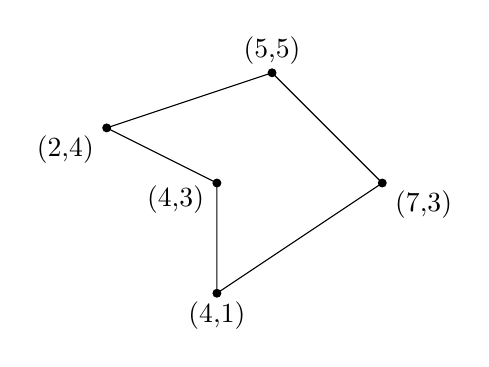
\begin{tikzpicture}[scale=0.7]
        \filldraw (4,1.4) circle (2pt);
        \filldraw (7,3.4) circle (2pt);
        \filldraw (5,5.4) circle (2pt);
        \filldraw (2,4.4) circle (2pt);
        \filldraw (4,3.4) circle (2pt);
        \node (1) at (4,1) {(4,1)};
        \node (2) at (7.75,3) {(7,3)};
        \node (3) at (5,5.8) {(5,5)};
        \node (4) at (1.25,4) {(2,4)};
        \node (5) at (3.25,3.1) {(4,3)};
        \path[draw] (4,1.4) -- (7,3.4) -- (5,5.4) -- (2,4.4) -- (4,3.4) -- (4,1.4);
    \end{tikzpicture}
\end{center}
es
\[\frac{\left|(2\cdot5-5\cdot4)+(5\cdot3-7\cdot5)+(7\cdot1-4\cdot3)+(4\cdot3-4\cdot1)+(4\cdot4-2\cdot3)\right|}{2} = 17/2.\]

La idea de la fórmula es recorrer trapezoides que comparten un lado con el
polígono y otro lado con la línea horizontal $y=0$. Por ejemplo:
\begin{center}
    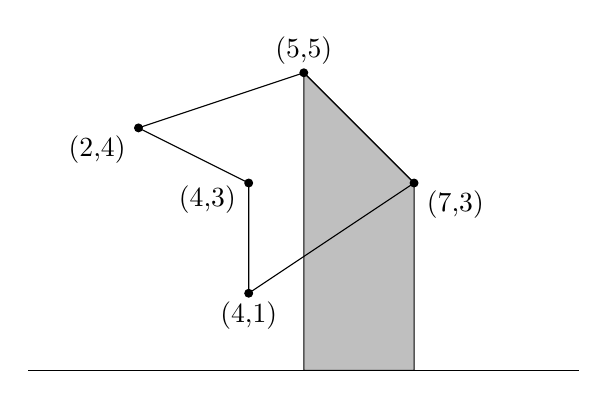
\begin{tikzpicture}[scale=0.7]
        \path[draw,fill=lightgray] (5,5.4) -- (7,3.4) -- (7,0) -- (5,0) -- (5,5.4);
        \filldraw (4,1.4) circle (2pt);
        \filldraw (7,3.4) circle (2pt);
        \filldraw (5,5.4) circle (2pt);
        \filldraw (2,4.4) circle (2pt);
        \filldraw (4,3.4) circle (2pt);
        \node (1) at (4,1) {(4,1)};
        \node (2) at (7.75,3) {(7,3)};
        \node (3) at (5,5.8) {(5,5)};
        \node (4) at (1.25,4) {(2,4)};
        \node (5) at (3.25,3.1) {(4,3)};
        \path[draw] (4,1.4) -- (7,3.4) -- (5,5.4) -- (2,4.4) -- (4,3.4) -- (4,1.4);
        \draw (0,0) -- (10,0);
    \end{tikzpicture}
\end{center}
El área de un trapezoide tal es
\[\left(x_{i+1}-x_{i}\right) \cdot \frac{y_i+y_{i+1}}{2},\]
donde los vértices del polígono son $p_i$ y $p_{i+1}$. Si $x_{i+1}>x_{i}$,
el área es positiva, y si $x_{i+1}<x_{i}$, el área es negativa.

El área del polígono es la suma de las áreas de todos estos trapezoides, lo
que resulta en la fórmula
\[\left|\,\sum_{i=1}^{n-1} (x_{i+1}-x_{i}) \cdot \frac{y_i+y_{i+1}}{2}\,\right| =
    \frac{1}{2} \left|\,\sum_{i=1}^{n-1} (x_i y_{i+1} - x_{i+1} y_i)\,\right|.\]

Cabe destacar que se debe tomar el valor absoluto de la suma, porque el valor
real puede ser positivo o negativo, dependiendo de si caminamos en sentido
horario o antihorario a través del borde del polígono.

\subsubsection{Teorema de Pick}

\index{teorema de!Pick}

El \key{teorema de Pick} nos da otra forma de calcular el área de un polígono,
dado que todos los vértices posean coordenadas enteras. Según el teorema de
Pick, el área del polígono es \[ a + \frac{b}{2} - 1,\] donde $a$ es el
número de puntos enteros ubicados dentro del polígono, y $b$ es el número de
puntos enteros ubicados en el borde del polígono.

Por ejemplo, el área del polígono
\begin{center}
    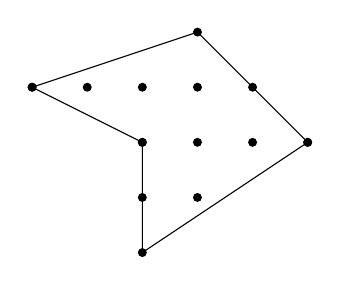
\begin{tikzpicture}[scale=0.7]
        \filldraw (4,1.4) circle (2pt);
        \filldraw (7,3.4) circle (2pt);
        \filldraw (5,5.4) circle (2pt);
        \filldraw (2,4.4) circle (2pt);
        \filldraw (4,3.4) circle (2pt);
        \path[draw] (4,1.4) -- (7,3.4) -- (5,5.4) -- (2,4.4) -- (4,3.4) -- (4,1.4);

        \filldraw (2,4.4) circle (2pt);
        \filldraw (3,4.4) circle (2pt);
        \filldraw (4,4.4) circle (2pt);
        \filldraw (5,4.4) circle (2pt);
        \filldraw (6,4.4) circle (2pt);

        \filldraw (4,3.4) circle (2pt);
        \filldraw (5,3.4) circle (2pt);
        \filldraw (6,3.4) circle (2pt);
        \filldraw (7,3.4) circle (2pt);

        \filldraw (4,2.4) circle (2pt);
        \filldraw (5,2.4) circle (2pt);
    \end{tikzpicture}
\end{center}
es $6+7/2-1=17/2$.

\section{Funciones de distancia}

\index{función de distancia}
\index{distancia euclideana}
\index{distancia de Manhattan}

Una \key{función de distancia} define la distancia entre dos puntos. La
función de distancia usual es la de \key{distancia euclideana}, que define la
distancia entre dos puntos $(x_1,y_1)$ y $(x_2,y_2)$ como
\[\sqrt{(x_2-x_1)^2+(y_2-y_1)^2}.\]
Una alternativa es la \key{distancia de Manhattan}, que define la distancia
entre los dos puntos como \[\left|x_1-x_2\right|+\left|y_1-y_2\right|.\]

Por ejemplo, considera la siguiente imagen:
\begin{center}
    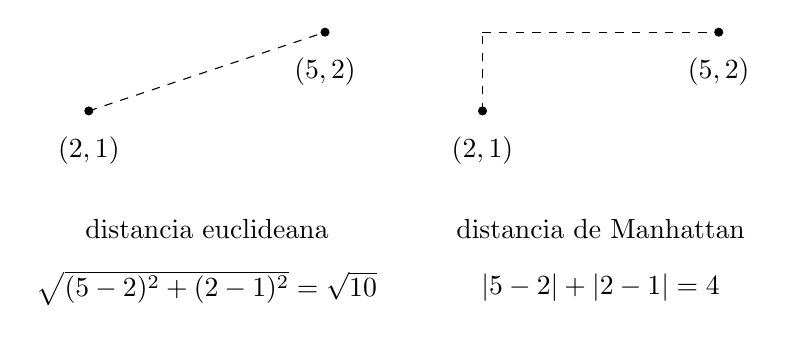
\begin{tikzpicture}

        \draw[fill] (2,1) circle [radius=0.05];
        \draw[fill] (5,2) circle [radius=0.05];

        \node at (2,0.5) {$(2,1)$};
        \node at (5,1.5) {$(5,2)$};

        \draw[dashed] (2,1) -- (5,2);

        \draw[fill] (5+2,1) circle [radius=0.05];
        \draw[fill] (5+5,2) circle [radius=0.05];

        \node at (5+2,0.5) {$(2,1)$};
        \node at (5+5,1.5) {$(5,2)$};

        \draw[dashed] (5+2,1) -- (5+2,2);
        \draw[dashed] (5+2,2) -- (5+5,2);

        \node at (3.5,-0.5) {distancia euclideana};
        \node at (3.5,-1.25) {$\sqrt{(5-2)^2+(2-1)^2}=\sqrt{10}$};
        \node at (5+3.5,-0.5) {distancia de Manhattan};
        \node at (5+3.5,-1.25) {$|5-2|+|2-1|=4$};
    \end{tikzpicture}
\end{center}

La siguiente imagen muestra regiones dentro de una distancia de 1 desde el
punto central, utilizando las distancias euclideana y de Manhattan:
\begin{center}
    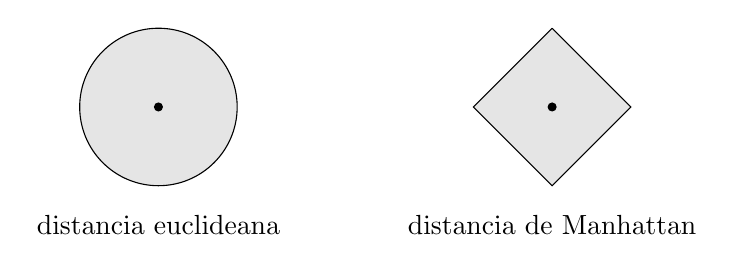
\begin{tikzpicture}

        \draw[fill=gray!20] (0,0) circle [radius=1];
        \draw[fill] (0,0) circle [radius=0.05];

        \node at (0,-1.5) {distancia euclideana};

        \draw[fill=gray!20] (5+0,1) -- (5-1,0) -- (5+0,-1) -- (5+1,0) -- (5+0,1);
        \draw[fill] (5,0) circle [radius=0.05];
        \node at (5,-1.5) {distancia de Manhattan};
    \end{tikzpicture}
\end{center}

\subsubsection{Rotar coordenadas}

Algunos problemas son más fáciles de resolver si usamos distancias de
Manhattan en vez de distancias euclideanas. Por ejemplo, considera un problema
donde recibimos $n$ puntos en el plano bidimensional y nuestra tarea es
calcular la máxima distancia de Manhattan entre cualquier par de puntos.

Por ejemplo, considera el siguiente conjunto de puntos:
\begin{center}
    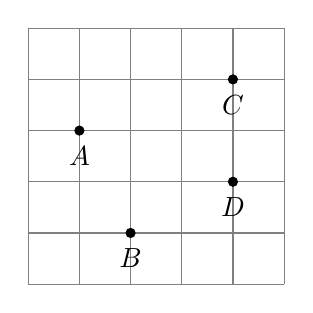
\begin{tikzpicture}[scale=0.65]
        \draw[color=gray] (-1,-1) grid (4,4);

        \filldraw (0,2) circle (2.5pt);
        \filldraw (3,3) circle (2.5pt);
        \filldraw (1,0) circle (2.5pt);
        \filldraw (3,1) circle (2.5pt);

        \node at (0,1.5) {$A$};
        \node at (3,2.5) {$C$};
        \node at (1,-0.5) {$B$};
        \node at (3,0.5) {$D$};
    \end{tikzpicture}
\end{center}
\pagebreak
La máxima distancia de Manhattan es 5, entre los puntos $B$ y $C$:
\begin{center}
    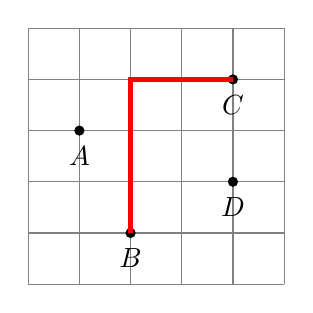
\begin{tikzpicture}[scale=0.65]
        \draw[color=gray] (-1,-1) grid (4,4);

        \filldraw (0,2) circle (2.5pt);
        \filldraw (3,3) circle (2.5pt);
        \filldraw (1,0) circle (2.5pt);
        \filldraw (3,1) circle (2.5pt);

        \node at (0,1.5) {$A$};
        \node at (3,2.5) {$C$};
        \node at (1,-0.5) {$B$};
        \node at (3,0.5) {$D$};

        \path[draw=red,thick,line width=2pt] (1,0) -- (1,3) -- (3,3);
    \end{tikzpicture}
\end{center}

Una técnica útil relacionada a las distancias de Manhattan es rotar todas
las coordenadas 45 grados tal que un punto $(x,y)$ se vuelve $(x+y,y-x)$.
Por ejemplo, luego de rotar los puntos de arriba, el resultado es:

\begin{center}
    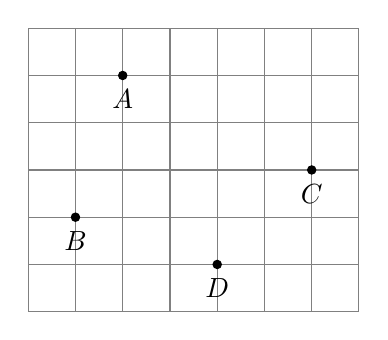
\begin{tikzpicture}[scale=0.6]
        \draw[color=gray] (0,-3) grid (7,3);

        \filldraw (2,2) circle (2.5pt);
        \filldraw (6,0) circle (2.5pt);
        \filldraw (1,-1) circle (2.5pt);
        \filldraw (4,-2) circle (2.5pt);

        \node at (2,1.5) {$A$};
        \node at (6,-0.5) {$C$};
        \node at (1,-1.5) {$B$};
        \node at (4,-2.5) {$D$};
    \end{tikzpicture}
\end{center}
Y la máxima distancia es la siguiente:
\begin{center}
    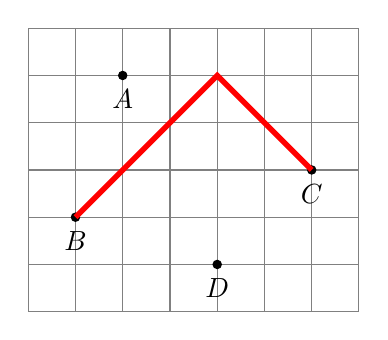
\begin{tikzpicture}[scale=0.6]
        \draw[color=gray] (0,-3) grid (7,3);

        \filldraw (2,2) circle (2.5pt);
        \filldraw (6,0) circle (2.5pt);
        \filldraw (1,-1) circle (2.5pt);
        \filldraw (4,-2) circle (2.5pt);

        \node at (2,1.5) {$A$};
        \node at (6,-0.5) {$C$};
        \node at (1,-1.5) {$B$};
        \node at (4,-2.5) {$D$};

        \path[draw=red,thick,line width=2pt] (1,-1) -- (4,2) -- (6,0);
    \end{tikzpicture}
\end{center}

Considera dos puntos $p_1=(x_1,y_1)$ y $p_2=(x_2,y_2)$ cuyas coordenadas
rotadas son $p'_1=(x'_1,y'_1)$ y $p'_2=(x'_2,y'_2)$. Ahora existen dos
formas de expresar la distancia de Manhattan entre $p_1$ y $p_2$:
\[|x_1-x_2|+|y_1-y_2| = \max(|x'_1-x'_2|,|y'_1-y'_2|)\]

Por ejemplo, si $p_1=(1,0)$ y $p_2=(3,3)$, las coordenadas rotadas son
$p'_1=(1,-1)$ y $p'_2=(6,0)$ y la distancia de Manhattan es
\[|1-3|+|0-3| = \max(|1-6|,|-1-0|) = 5.\]

Las coordenadas rotadas brindan una simple forma de operar con las distancias
de Manhattan, porque podemos considerar coordenadas $x$ e $y$ separadamente.
Para maximizar la distancia de Manhattan entre dos puntos, deberíamos
encontrar dos puntos cuyas coordenadas rotadas maximizan el valor de
\[\max(|x'_1-x'_2|,|y'_1-y'_2|).\]
Esto es fácil, porque o la diferencia horizontal o la vertical entre las
coordenadas rotadas debe ser máxima.
